\documentclass[extra,mreferee]{gji}
%\documentclass[extra,onecolumn,doublespacing]{gji}
\usepackage{timet}
\usepackage{amsmath}
\usepackage{amsfonts}
\usepackage{amssymb}
\usepackage{graphicx}
\usepackage{arydshln}
\usepackage{bm}
\usepackage{ulem}

\title[Transient strain in geodetic data]
      {Revealing transient strain in geodetic data with Gaussian process regression}

\author[T. T. Hines and E. A. Hetland]
       {T. T. Hines$^1$ and E. A. Hetland$^1$ \\
        $^1$ Department of Earth and Environmental Sciences, University of Michigan, Ann Arbor, MI, USA}

\date{Received XXX; in original form XXX}

\pagerange{\pageref{firstpage}--\pageref{lastpage}}

\volume{XXX}

\pubyear{XXX}

% Authors with AMS fonts and mssymb.tex can comment out the following
% line to get the correct symbol for Geophysical Journal International.
\let\leqslant=\leq

\newtheorem{theorem}{Theorem}[section]

\begin{document}

\label{firstpage}

\maketitle

\begin{summary}
Transient strain rates derived from GNSS data can be used to detect and understand geophysical phenomena such as slow slip events and postseismic deformation. Here we propose using Gaussian process regression (GPR) as a tool for estimating transient strain rates from GNSS data. GPR is a non-parametric, Bayesian method for interpolating scattered data. Transient strain rates estimated with GPR have meaningful uncertainties, allowing geophysical signal to be easily discerned from noise. In our approach, we assume a stochastic prior model for transient displacements. The prior describes how much one expects transient displacements to covary spatially and temporally. A posterior estimate of transient strain rates is obtained by differentiating the posterior displacements. One limitation with GPR is that it is not robust against outliers, so we introduce a pre-processing method for detecting and removing outliers in GNSS data. As a demonstration, we use GPR to detect transient strain resulting from slow slip events in Cascadia. Maximum likelihood methods are used to constrain a prior model for transient displacements in this region. The temporal covariance of our prior model is described by a compact Wendland covariance function, which significantly reduces the computational burden that can be associated with GPR. Our results reveal the spatial and temporal evolution of strain from slow slip events. We verify that the transient strain estimated with GPR is in fact geophysical signal by comparing it to the seismic tremor that is associated with Cascadia slow slip events.
\end{summary}

\begin{keywords}
 XXX -- XXX -- XXX -- XXX.
\end{keywords}

\section{Introduction}\label{sec:Introduction}
Crustal strain rates are fundamentally important quantities for assessing seismic hazard. Knowing where and how quickly strain is accumulating gives insight into where we can expect stored elastic energy to be released seismically. Consequently, secular crustal strain rates estimated from GNSS data have been used to constrain seismic hazard models such as UCERF3 \citep{Field2014}. Transient crustal strain, which is caused by geophysical phenomena such as slow slip events (SSEs) or postseismic deformation, is also relevant for assessing seismic hazard. While transient strain itself is not damaging, there is a risk that it can trigger major earthquakes \citep{Roeloffs2006,Freed2001}. Dense networks of continuous GNSS stations, such as the Plate Boundary Observatory (PBO), make it possible to identify transient strain with high fidelity. Developing and improving upon methods for deriving secular and transient strain from GNSS data is an active area of research.

Most methods for estimating strain rates from GNSS data assume some parametric form of the deformation signal. The simplest method for estimating secular strain rates assumes that GNSS derived velocities can be described with a first-order polynomial (i.e., having constant deformation gradients) over some subnetwork of the GNSS stations \citep[e.g.,][]{Feigl1990,Murray2000}. The components of the strain rate tensor  for each subnetwork are then determined through a least squares fit to the observations. The assumption that deformation gradients are spatially uniform is not appropriate when subnetworks span too large of an area. To help overcome this deficiency, \citet{Shen1996,Shen2015} used an inverse distance weighting scheme, in which the estimated strain rate at some point is primarily controlled by observations at nearby stations. However, the methods described in \citet{Shen1996,Shen2015} are still formulated by assuming that the deformation gradients are uniform over the entire network. The errors in this assumption manifest as implausibly low formal uncertainties for the estimated strain rates. Other methods for estimating secular strain rates have parameterized GNSS derived velocities with bi-cubic splines \citep{Beavan2001}, spherical wavelets \citep{Tape2009}, and elastostatic Green's functions \citep{Sandwell2016}. The type of basis functions and the number of degrees of freedom for a parameterization can be subjective. If there are too few degrees of freedom in the parameterization, then estimated strain rates will be biased and the uncertainties will be underestimated. On the other hand, if there are too many degrees of freedom, then there will not be any coherent features in the estimated strain rates. The methods described by \citet{Beavan2001} and \citet{Tape2009} also require the user to specify penalty parameters that control a similar trade-off between bias and variance in the solution. One could parameterize deformation with a physically motivated model of interseismic deformation \citep[e.g.,][]{Meade2005,McCaffrey2007}. In such models the lithospheric rheology and fault geometries are assumed to be known. Any errors in the assumed physical model could result in biased strain estimates and underestimated formal uncertainties. 

The aforementioned studies are concerned with estimating secular strain rates. In recent years the Southern California Earthquake Center (SCEC) community has shown interest in developing methods for detecting transient strain. SCEC supported a transient detection exercise \citep{Lohman2013}, where several research groups tested their methods for detecting transient geophysical signal with a synthetic GNSS dataset. Among the methods tested were the Network Strain Filter (NSF) \citep{Ohtani2010} and the Network Inversion Filter (NIF) \citep{Segall1997}. The NSF uses a wavelet parameterization to  describe the spatial component of geophysical signal. The NIF, which is intended for imaging slow fault slip from geodetic data, uses the elastic dislocation Green's functions from \citet{Okada1992}. For the NSF and NIF, the time dependence of the geophysical signal is modeled as integrated Brownian motion. The method described in \citet{Holt2013} was also tested in the SCEC transient detection exercise, which calculates strain rates using a bi-cubic spatial parameterization of displacements between time epochs. \citet{Holt2013} defined a detection threshold based on the strain rate magnitude, and below we demonstrate that this is indeed an effective criterion for identifying geophysical signal. For the same reasons descibed above, the transient deformation and corresponding uncertainties estimated by these methods can be biased by the chosen spatial parameterization. It is then difficult to distinguish signal from noise with these methods, which limits their utility for transient detection.   

Here we propose using Gaussian process regression (GPR) \citep{Rasmussen2006} to estimate transient strain from GNSS data. GPR is a Bayesian, non-parametric method for inferring a continuous signal from scattered data. Since GNSS stations are irregularly spaced and observation times may differ between stations, GPR is an ideal tool for synthesizing GNSS data into a spatially and temporally continuous representation of surface deformation. GPR is closely related to kriging \citep{Cressie1992} and least squares collocation \citep{Moritz1978}. The latter has been used by \citet{Kato1998} and \citet{El-Fiky1999} to estimate secular strain rates from GNSS data. GPR is Bayesian in that we describe our prior understanding of the geophysical signal with a Gaussian process. A Gaussian process is a normally distributed stochastic process that is fully defined in terms of a mean function and a positive definite covariance function. For example, Brownian motion, $B(t)$, is a well known Gaussian process in $\mathbb{R}^1$ which has zero mean and covariance function $\mathrm{cov}(B(t),B(t')) = \min(t,t')$, where $t,t' \ge 0$. If no prior information is available for the geophysical signal, then maximum likelihood methods can be used to objectively choose a prior Gaussian process that is most consistent with the observations.  We incorporate GNSS observations with the prior to form a posterior estimate of transient strain.  The posterior transient strain is also a Gaussian process, and we can use its distribution to confidently discern geophysical signal from noise. We use GPR to infer strain resulting from SSEs in Cascadia, demonstrating that GPR is an effective tool for detecting transient geophysical processes. 

\section{Estimating Transient Strain Rates}\label{sec:Method}
We seek a spatially and temporally dependent estimate of transient crustal strain rates. We consider transient strain rates to be any deviation from secular strain rates, and our attention is limited to horizontal strain rates in this study. We denote transient crustal strain rates as $\dot\varepsilon(p)$, where $p$ represents the ordered pair $(\vec{x},t)$, $\vec{x}$ are spatial coordinates in $\mathbb{R}^2$, and $t$ is time. We determine $\dot\varepsilon(p)$ by spatially and temporally differentiating estimates of transient displacements, $\vec{u}(p)$. We make a prior assumption that each component of $\vec{u}$ is a Gaussian process,
\begin{equation}\label{eq:TransientDeformation}
u_i(p) \sim \mathcal{N}\left(0,C_{u_i}\right),
\end{equation}
where $C_{u_i}(p,p')$ is a covariance function indicating how we expect $u_i(p)$ to covary with $u_i(p')$. For simplicity, we treat each component of displacements independently and ignore any potential covariance between them. Hence, we drop the component subscripts with the understanding that the same analysis is being repeated to estimate the easting and northing components of $\vec{u}$. We assume that $C_u$ can be separated into spatial and temporal functions as 
\begin{equation}\label{eq:TransientCovariance}
C_{u}\left((\vec{x},t),(\vec{x}',t')\right) = X(\vec{x},\vec{x}')T(t,t').
\end{equation}  
As long as the functions $X$ and $T$ are positive definite, $C_u$ is guaranteed to also be positive definite and thus a valid covariance function \citep[sec. 4.2.4]{Rasmussen2006}. The appropriate choice for $X$ and $T$ may vary depending on the geophysical signal we are trying to describe, and we discuss this matter in Section \ref{sec:SignalModel}.  

We constrain $u$ with GNSS data, which records $u$ as well as other physical and non-physical processes that we are not interested in. We describe GNSS observations at position $\vec{x}_i$ and time $t_j$ as a realization of the random variable 
\begin{align}\label{eq:Data}
\begin{split}
d_{ij} = &u(\vec{x}_i,t_j) + \eta(\vec{x}_i,t_j) + w_{ij} + a^{(1)}_i + a^{(2)}_it_j + \\
         &a^{(3)}_i\sin(2 \pi t_j) + a^{(4)}_i\cos(2 \pi t_j) + a^{(5)}_i\sin(4 \pi t_j) + a^{(6)}_i\cos(4 \pi t_j), 
\end{split}
\end{align}
where $a^{(1)}_{i}$ is an offset that is unique for each GNSS monument, $a^{(2)}_{i}$ is the secular velocity at $\vec{x}_i$, and the sinusoids describe seasonal deformation (using units of years for $t_j$). We use $w_{ij}$ to denote normally distributed, uncorrelated noise. Correlated noise which does not have a parametric representation is denoted by $\eta$.  For example, $\eta$ can consist of temporally correlated noise describing benchmark wobble \citep[e.g.,][]{Wyatt1982,Wyatt1989}, and/or spatially correlated noise describing common mode error \citep[e.g.,][]{Wdowinski1997}. For now, we will only assume that $\eta \sim \mathcal{N}(0,C_\eta)$. We consider the six coefficients in eq. (\ref{eq:Data}) to be uncorrelated random variables distributed as $\mathcal{N}(0,\kappa^2)$ in the limit as $\kappa \to \infty$ (i.e., the coefficients have diffuse priors). Of course, the secular velocities, $a^{(2)}_{i}$, are spatially correlated and we could invoke a tectonic model to form a prior on $a^{(2)}_{i}$. However, in our application to Cascadia, we will be using displacement time series which are long enough to sufficiently constrain $a^{(2)}_{i}$ for each station, avoiding the need to incorporate a prior. Likewise, seasonal deformation is spatially correlated \citep{Dong2002,Langbein2008}, and it may be worth exploring and exploiting such a correlation in a future study. 

We now consider the column vector of $n$ GNSS observations made at $m$ stations, $\mitbf{d}_*$. Let $\mitbf{P}$ be the set of $(\vec{x}_i, t_j)$ pairs describing where and when each of the GNSS observations have been made. Let $\mitbf{a}$ be the vector of coefficients from eq. (\ref{eq:Data}) for each of the $m$ GNSS stations. We use $\mitbf{G}$ to represent the $n \times 6m$ matrix of corresponding basis functions evaluated at each point in $\mitbf{P}$. We  also denote the vector of uncorrelated noise for each observation as $\mitbf{w}$, whose standard deviations are given by the formal data uncertainty, $\mitbf{\sigma}$. The observations can then be viewed as a realization of the random vector
\begin{equation}
\mitbf{d} = u(\mitbf{P}) + \eta(\mitbf{P}) + \mitbf{w} + \mitbf{G}\mitbf{a},
\end{equation}
which is distributed as $\mathcal{N}(\mitbf{0},\mitbf{\Sigma} + \kappa^2\mitbf{G}\mitbf{G}^T)$, where
\begin{equation}\label{eq:Cd}
\mitbf{\Sigma} = C_u(\mitbf{P},\mitbf{P}) + C_\eta(\mitbf{P},\mitbf{P}) + 
              \mathrm{diag}\left(\mitbf{\sigma}^2\right).  
\end{equation}
It should be understood that notation such as $u(\mitbf{P})$ and $C_u(\mitbf{P},\mitbf{P})$ represents the column vector $[u(P_i)]_{P_i \in \mitbf{P}}$ and the matrix $[C_u(P_i,P_j)]_{(P_i,P_j) \in \mitbf{P} \times \mitbf{P}}$, respectively. 

The prior for transient displacements is then conditioned with $\mitbf{d}_*$ to form a posterior estimate of transient displacements, $\hat{u} = u | \mitbf{d}_*$. For now, we will assume that appropriate covariance functions and corresponding hyperparameters for $C_u$ and $C_\eta$ have already been chosen. In Section \ref{sec:NoiseModel} and \ref{sec:SignalModel}, we discuss how the covariance functions are chosen for our application to GNSS data from Cascadia. If $\kappa$ is kept finite then, from \citet[sec. 2.2]{Rasmussen2006}, we find that $\hat{u}$ is distributed as $\mathcal{N}(\mu_{\hat{u}},C_{\hat{u}})$, where
\begin{equation}\label{eq:PosteriorMean}
\mu_{\hat{u}}(p) = C_u(p,\mitbf{P})\left(\mitbf{\Sigma} + \kappa^2\mitbf{G}\mitbf{G}^T\right)^{-1}\mitbf{d}_*
\end{equation}    
and
\begin{equation}\label{eq:PosteriorCov}
C_{\hat{u}}(p,p') = C_u(p,p') - C_u(p,\mitbf{P})\left(\mitbf{\Sigma} + \kappa^2\mitbf{G}\mitbf{G}^T\right)^{-1}C_u(\mitbf{P},p').
\end{equation}
However, we are interested in the limit as $\kappa \to \infty$, and the form for eq. (\ref{eq:PosteriorMean}) and eq. (\ref{eq:PosteriorCov}) is not suitable for evaluating this limit. We use a partitioned matrix inversion identity \citep[sec. 2.7.4]{Press2007} to rewrite eq. (\ref{eq:PosteriorMean}) and eq. (\ref{eq:PosteriorCov}) as
 \begin{equation}\label{eq:PosteriorMean2}
\mu_{\hat{u}}(p) = \left[\begin{array}{cc}
                         C_u(p,\mitbf{P}) & \mitbf{0} \\
                         \end{array}\right]
                   \left[\begin{array}{cc}
                         \mitbf{\Sigma} & \mitbf{G} \\
                         \mitbf{G}^T  & -\kappa^{-2} \mitbf{I} \\
                         \end{array}\right]^{-1}
                   \left[\begin{array}{c}
                         \mitbf{d}_* \\
                         \mitbf{0} \\
                         \end{array}\right]
\end{equation}    
and
\begin{equation}\label{eq:PosteriorCov2}
C_{\hat{u}}(p,p') = C_u(p,p') - 
                    \left[\begin{array}{cc}
                          C_u(p,\mitbf{P}) & \mitbf{0} \\
                          \end{array}\right]
                    \left[\begin{array}{cc}
                          \mitbf{\Sigma} & \mitbf{G} \\
                          \mitbf{G}^T  & -\kappa^{-2} \mitbf{I} \\
                          \end{array}\right]^{-1}
                    \left[\begin{array}{c}
                          C_u(\mitbf{P},p') \\
                          \mitbf{0} \\
                          \end{array}\right].
\end{equation}
Taking the limit as $\kappa \to \infty$, we get the solution for the mean and covariance of $\hat{u}$,
 \begin{equation}\label{eq:PosteriorMean3}
\mu_{\hat{u}}(p) = \left[\begin{array}{cc}
                         C_u(p,\mitbf{P}) & \mitbf{0} \\
                         \end{array}\right]
                   \left[\begin{array}{cc}
                         \mitbf{\Sigma} & \mitbf{G} \\
                         \mitbf{G}^T  & \mitbf{0} \\
                         \end{array}\right]^{-1}
                   \left[\begin{array}{c}
                         \mitbf{d}_* \\
                         \mitbf{0} \\
                         \end{array}\right]
\end{equation}    
and
\begin{equation}\label{eq:PosteriorCov3}
C_{\hat{u}}(p,p') = C_u(p,p') - 
                    \left[\begin{array}{cc}
                          C_u(p,\mitbf{P}) & \mitbf{0} \\
                          \end{array}\right]
                    \left[\begin{array}{cc}
                          \mitbf{\Sigma} & \mitbf{G} \\
                          \mitbf{G}^T  & \mitbf{0} \\
                          \end{array}\right]^{-1}
                    \left[\begin{array}{c}
                          C_u(\mitbf{P},p') \\
                          \mitbf{0} \\
                          \end{array}\right].
\end{equation}

We use eq. (\ref{eq:PosteriorMean3}) and (\ref{eq:PosteriorCov3}) to find the posterior easting and northing components of transient displacements. Using $\hat{u}_i$ to denote the posterior transient displacements along direction $i$ and $x_i$ to represent the components of $\vec{x}$, we can write the components of $\dot\varepsilon$ as 
\begin{equation}\label{eq:StrainRate}
\dot\varepsilon_{ij}(p) = \frac{1}{2} \frac{\partial}{\partial t} \left(
                                        \frac{\partial \hat{u}_i(p)}{\partial x_j} +  
                                        \frac{\partial \hat{u}_j(p)}{\partial x_i}\right).
\end{equation}
The transient strain rate components are stochastic processes whose distributions can be interpreted as the distributions of samples of $\hat{u}$ that have been differentiated by the operator from eq. (\ref{eq:StrainRate}). Since differentiation is a linear operation, the transient strain rate components are Gaussian processes. From \citet[sec. 10.2]{Papoulis1991}, we find that the components of $\dot{\varepsilon}$ have mean functions
\begin{equation}\label{eq:StrainMean}
\mu_{\dot\varepsilon_{ij}}(p) = \frac{1}{2}\frac{\partial}{\partial t}\left(
                                  \frac{\partial \mu_{\hat{u}_i}(p)}{\partial x_j} + 
                                  \frac{\partial \mu_{\hat{u}_j}(p)}{\partial x_i} \right)
\end{equation} 
and covariance functions
\begin{equation}\label{eq:StrainCov}
C_{\dot\varepsilon_{ij}}(p,p') = \frac{1}{4} \frac{\partial^2}{\partial t \, \partial t'}\left(
                                   \frac{\partial^2 C_{\hat{u}_i}(p,p')}{\partial x_j \, \partial x'_j} + 
                                   \frac{\partial^2 C_{\hat{u}_j}(p,p')}{\partial x_i \, \partial x'_i} \right).
\end{equation} 

Our motivation for estimating transient strain rates is, in part, to detect geophysical phenomena. We propose using a signal-to-noise ratio, SNR, based on $\dot\varepsilon$ for our detection criterion. The Frobenius norm of $\dot\varepsilon$, $||\dot\varepsilon||_\mathrm{F}$, which is sometimes referred to as the second invariant of strain rate in the geodetic literature, is often used as a metric for the strain rate ``magnitude''. Noting that $||\dot\varepsilon||_\mathrm{F}$ is a random variable, SNR can be taken as the ratio of the estimated mean and standard deviation of $||\dot\varepsilon||_\mathrm{F}$. Using nonlinear uncertainty propagation, we find SNR to be  
\begin{equation}\label{eq:SNR}
\mathrm{SNR}(p) = \frac{\mu_{\dot\varepsilon_\mathrm{nn}}(p)^2 +
                        \mu_{\dot\varepsilon_\mathrm{ee}}(p)^2 +
                        2\mu_{\dot\varepsilon_\mathrm{en}}(p)^2}
                       {\big(C_{\dot\varepsilon_\mathrm{nn}}(p,p)\mu_{\dot\varepsilon_\mathrm{nn}}(p)^2 + 
                              C_{\dot\varepsilon_\mathrm{ee}}(p,p)\mu_{\dot\varepsilon_\mathrm{ee}}(p)^2 + 
                              4C_{\dot\varepsilon_\mathrm{en}}(p,p)\mu_{\dot\varepsilon_\mathrm{en}}(p)^2
                        \big)^{\frac{1}{2}}}
,
\end{equation}
where the subscripts ``n'' and ``e'' denote north and east, respectively. For simplicity, we have ignored covariances between the transient strain rate components in eq. (\ref{eq:SNR}), even though they are non-zero.  

\section{Outlier detection}\label{sec:Outlier}
In our formulation for estimating transient strain rates, we have assumed that noise in the data vector is normally distributed. This is not an appropriate assumption for GNSS data, which often have more outliers than would be predicted for normally distributed noise. It follows that proposed methods for analyzing GNSS data should be robust against outliers \citep[e.g.,][]{Blewitt2016}. In order to make our estimates of transient strain more robust, we automatically identify and remove outliers in the GNSS data as a pre-processing step.

Our method for detecting outliers is based on the data editing algorithm described in \citet{Gibbs2011}. We calculate the residuals between the observations and a best fitting model. Data with residuals that are anomalously large are then identified as outliers. We treat $\mitbf{d}_*$ as a sample of $\mitbf{d}$ and assume that there is no correlated noise (i.e., $\eta(p) = 0$).  The best fitting model for $\mitbf{d}_*$ is considered to be the expected value of the random vector $u(\mitbf{P}) + \mitbf{G}\mitbf{a}$ after conditioning it with non-outlier observations.  We still consider $u$ to have a separable covariance function as in eq. (\ref{eq:TransientCovariance}), and the choice for $X$ and $T$ does not need to be the same as that used in Section \ref{sec:Method}. Since outliers are determined based on how well a spatially and temporally dependent model fits the data, we are able to identify anomalous observations which may not be immediately apparent from inspecting individual time series. 

To begin the algorithm, we let $\mitbf{\Omega}$ be the index set of non-outliers in $\mitbf{d}_*$ and initiate it with all $n$ indices. This algorithm is iterative, and for each iteration we calculate the residual vector
\begin{align}\label{eq:Residual}
\mitbf{r} &= \frac{\mitbf{d}_* - \mathrm{E}\left[(u(\mitbf{P}) + \mitbf{G}\mitbf{a})|\tilde{\mitbf{d}}_* \right]}{\mitbf{\sigma}} \\
       &= \frac{1}{\mitbf{\sigma}}\left(\mitbf{d}_*  - 
          \left[\begin{array}{cc}
                C_u(\mitbf{P},\tilde{\mitbf{P}}) & \mitbf{G} \\
                \end{array}\right]
          \left[\begin{array}{cc}
                C_u(\tilde{\mitbf{P}},\tilde{\mitbf{P}}) + \mathrm{diag}(\tilde{\mitbf{\sigma}}^2) & \tilde{\mitbf{G}} \\
                \tilde{\mitbf{G}}^T  & \mitbf{0} \\
                \end{array}\right]^{-1}
          \left[\begin{array}{c}
                \tilde{\mitbf{d}}_* \\
                \mitbf{0} \\
                \end{array}\right]\right),
\end{align}
where the tilde indicates that only elements corresponding to indices in $\mitbf{\Omega}$ are retained (e.g., $\tilde{\mitbf{P}} = \{P_i\}_{i\in\mitbf{\Omega}}$). We then update $\mitbf{\Omega}$ to be
\begin{equation}\label{eq:Update}
\mitbf{\Omega} = \{i : |r_i| < \lambda \cdot \mathrm{RMS}\}, \ \ \ r_i \in \mitbf{r},
\end{equation} 
where RMS is the root-mean-square of $\tilde{\mitbf{r}}$ and $\lambda$ is an outlier tolerance. We use $\lambda=4$ in this study, which in our experience accurately identifies outliers without unnecessarily decimating the data. Iterations continue until the new $\mitbf{\Omega}$ is equal to the previous $\mitbf{\Omega}$. 

It should be noted that this algorithm does not identify jumps in GNSS time series, which are another common issue. Some, but not all, jumps can be automatically removed by looking up the dates of equipment changes and earthquakes. However, it is still necessary to manually find and remove jumps of unknown origin. That being said, this outlier detection algorithm significantly reduces the effort needed to manually clean GNSS data.       

\section{Application to Cascadia Slow Slip Events}\label{sec:Cascadia}
We use our method to estimate transient strain rates in Cascadia, and we are specifically interested in identifying strain resulting from SSEs \citep[e.g.,][]{Dragert2001}. In Cascadia, SSEs can be detected by monitoring for associated seismic tremor \citep{Rogers2003}, which is actively being done by the Pacific Northwest Seismic Network \citep{Wech2010}. We can thus compare the tremor records to the transient strain rates estimated with GPR to verify that we are indeed identifying strain from SSEs.  

We use the daily displacement solutions generated by the Geodesy Advancing Geosciences and EarthScope (GAGE) facility for continuous GNSS stations \citep{Herring2016}. This data is publicly available and can be found at www.unavco.org. We limit the dataset to the stations and time ranges which are pertinent to the seven most recent SSEs in the Puget Sound region. The earliest SSE considered in this study began in August 2010, and the most recent SSE began in February 2017. We use these most recent SSEs because the station coverage is sufficiently dense for us to use maximum likelihood methods to constrain prior models.  The positions of GNSS stations used to estimate transient strain rates are shown in Figure \ref{fig:Context}.  

\begin{figure*}
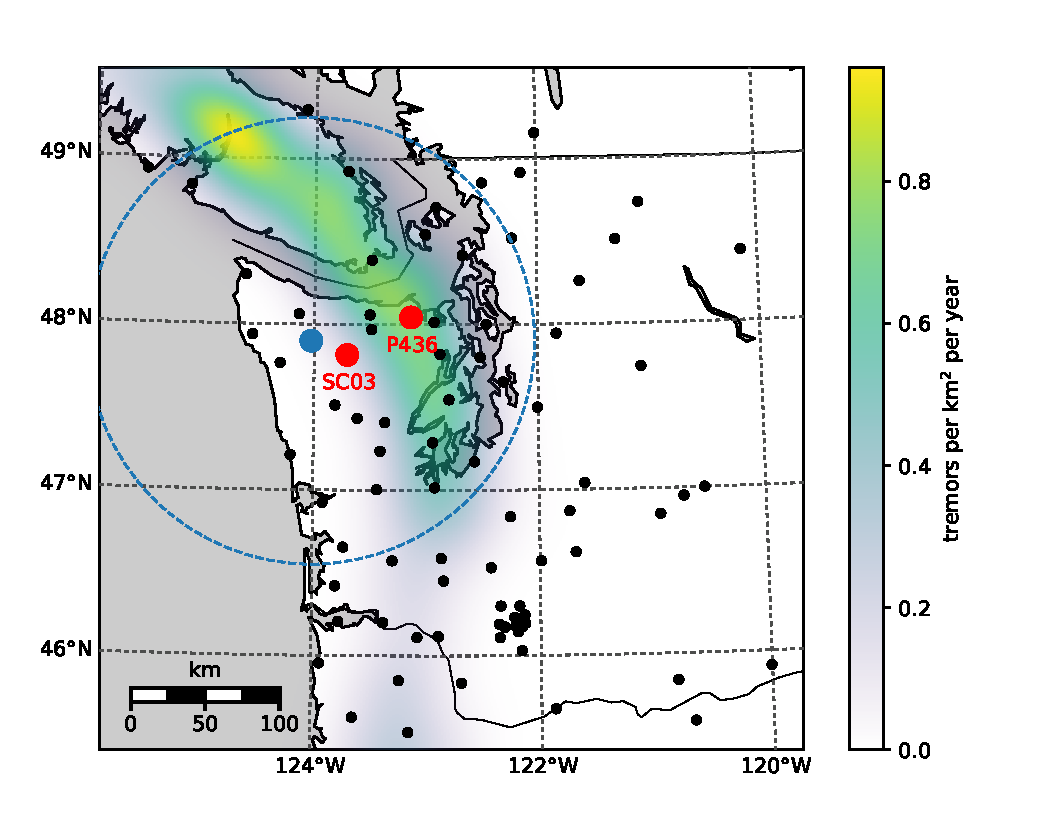
\includegraphics{figures/context_map/context-map.pdf}
\caption{Positions of continuous GNSS stations used to estimate transient strain rates. The colored regions indicate the distribution of seismic tremor as determined by \citet{Wech2010}. The red dots show the positions of GNSS stations mentioned in this paper. The blue dot indicates the location of the transient strain rates shown in Figure \ref{fig:StrainTs} and the signal-to-noise ratio shown in Figure \ref{fig:StrainMag}. The blue dashed circle demarcates the spatial extent of the tremors shown in Figure \ref{fig:StrainMag}.}    
\label{fig:Context}
\end{figure*}

\subsection{Noise model}\label{sec:NoiseModel}
Before we determine the transient strain rates, we must establish a prior for the transient displacements, $u$, and the noise, $\eta$. In this section we discuss our choice for the noise covariance function $C_\eta$. There have been numerous studies on temporally correlated noise in GNSS data \citep[e.g.,][]{Zhang1997,Mao1999,Williams2004,Langbein2008}. In these studies, temporally correlated noise was described with some combination of Brownian motion, a first-order Gauss-Markov (FOGM) process, and/or flicker noise. There is some physical justification for using Brownian motion as a noise model because it accurately describes the power spectrum of motion resulting from instability in geodetic monuments \citep[e.g.,][]{Wyatt1982,Wyatt1989}. Here we describe the time dependence of $\eta$ as a FOGM process and consider $\eta$ to be spatially uncorrelated. A FOGM process is a solution to the stochastic differential equation
\begin{equation}\label{eq:FOGMdef}
\dot{\eta}(t) + \alpha \eta(t) = \beta w(t),
\end{equation}
where $w(t)$ is white noise with unit variance. The FOGM process degenerates to the commonly used Brownian motion noise model under the condition that $\alpha=0$ and $\eta(0) = 0$. Our noise model that satisfies eq. (\ref{eq:FOGMdef}) is a Gaussian process with zero mean and the covariance function
\begin{equation}\label{eq:FOGM}
C_\eta\left((\vec{x},t),(\vec{x}',t')\right) = \frac{\beta^2}{2\alpha}\exp\left(-\alpha|t - t'|\right) \delta(||\vec{x} - \vec{x}'||_2). 
\end{equation}

We constrain the hyperparameters for $\eta$, $\alpha$ and $\beta$, with a set of 38 continuous GNSS stations in Cascadia that are east of 121$^\circ$W.  These stations are sufficiently far from the subduction zone that they are unlikely to contain transient signal associated with SSEs.  We clean the data for these stations by removing jumps at times of equipment changes, and we remove outliers that have been detected with the algorithm described in Section \ref{sec:Outlier}. We then find $\alpha$ and $\beta$ for each station time series with the Restricted Maximum Likelihood (REML) method \cite[e.g.,][]{Harville1974,Cressie1992,Hines2017}. The REML method finds the hyperparameters, which we collectively refer to as $\mitbf{\theta}$, that maximize the likelihood function
\begin{equation}\label{eq:REML}
\mathcal{L}(\mitbf{\theta}) = \left(\frac{\left|\mitbf{G}^T\mitbf{G}\right|}
                           {(2\pi)^{n-6m} 
                           \left| \mitbf{\Sigma}(\mitbf{\theta}) \right| 
                           \left| \mitbf{G}^T\mitbf{\Sigma}(\mitbf{\theta})^{-1}\mitbf{G} \right|}\right)^{\frac{1}{2}} 
                           e^{-\tfrac{1}{2}\mitbf{d}_*^T\mitbf{K}(\mitbf{\theta})\mitbf{d}_*},
\end{equation}
where
\begin{equation}
\mitbf{K}(\mitbf{\theta}) = \mitbf{\Sigma}(\mitbf{\theta})^{-1} - 
                      \mitbf{\Sigma}(\mitbf{\theta})^{-1}\mitbf{G}
         \left(\mitbf{G}^T\mitbf{\Sigma}(\mitbf{\theta})^{-1}\mitbf{G}\right)^{-1}
         \mitbf{G}^T\mitbf{\Sigma}(\mitbf{\theta})^{-1}.
\end{equation}
\citet{Harville1974} showed that choosing the hyperparameters which maximize eq. (\ref{eq:REML}) is equivalent to choosing the hyperparameters which maximize the probability of drawing $\mitbf{d}_*$ from $\mitbf{d}$. We use the REML method over the maximum likelihood method \citep[e.g.,][]{Langbein1997} because the REML method accounts for the improper prior that we assigned to $\mitbf{a}$ \citep{Hines2017}. We independently estimate $\mitbf{\theta}$ for each station, and so $\mitbf{d}_*$ consists of displacements for an individual station. We are assuming $u(p)=0$ when estimating the noise hyperparameters for this section. The distribution of inferred $\alpha$ and $\beta$ are shown in Figure \ref{fig:NoiseParams}. The amplitude of FOGM noise, $\beta$, for the easting and northing components is notable low and are clustered around 0.5 mm/yr$^{0.5}$. The corresponding estimates of $\alpha$ tend to cluster around 0 yr$^{-1}$, suggesting that noise can be described with Brownian motion. We also estimate hyperparameters for the vertical component of displacements, under the hope that vertical deformation gradients could reveal some geophysical signal. The amplitude of FOGM noise for the vertical component is relatively large with a median value of 13.5 mm/yr$^{0.5}$.  The inferred values for $\alpha$ are also higher for the vertical component with a median value of 8.21 yr$^{-1}$. In Figure \ref{fig:NoiseSamples}, we use the median values of $\alpha$ and $\beta$ to generate two random samples of FOGM noise for each component. The samples span five years and over these five years the easting and northing samples drift by about 1 mm. In the context of detecting SSEs, which produce several mm's of surface displacement on the time-scale of weeks, the estimated FOGM noise for the easting and northing component is negligible. In contrast, the estimated FOGM noise for the vertical component is larger than the signal we would expect from SSEs. We suspect that the higher amplitude for the FOGM noise in the vertical component is accommodating for deficiencies in our rather simple seasonal model. Based on this analysis, we henceforth ignore temporally correlated noise in the easting and northing component because of its low amplitude. We also do not use vertical displacements because of the presumably low signal-to-noise ratio.

\begin{figure*}
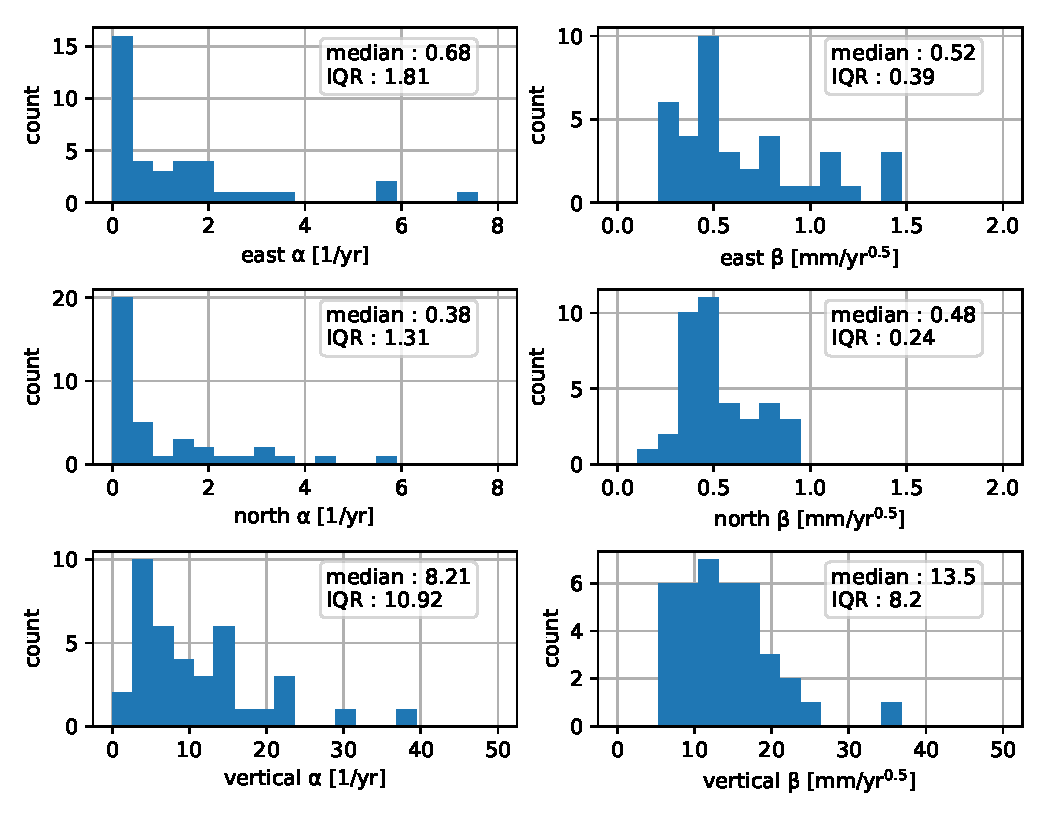
\includegraphics{figures/noise/noise-params.pdf}
\caption{Distribution of estimated FOGM hyperparameters (eq. \ref{eq:FOGM}). Hyperparameters are estimated with the REML method for 38 stations in Cascadia that are east of $121^\circ$W. ``IQR'' is the interquartile range.}   
\label{fig:NoiseParams}
\end{figure*}

\begin{figure*}
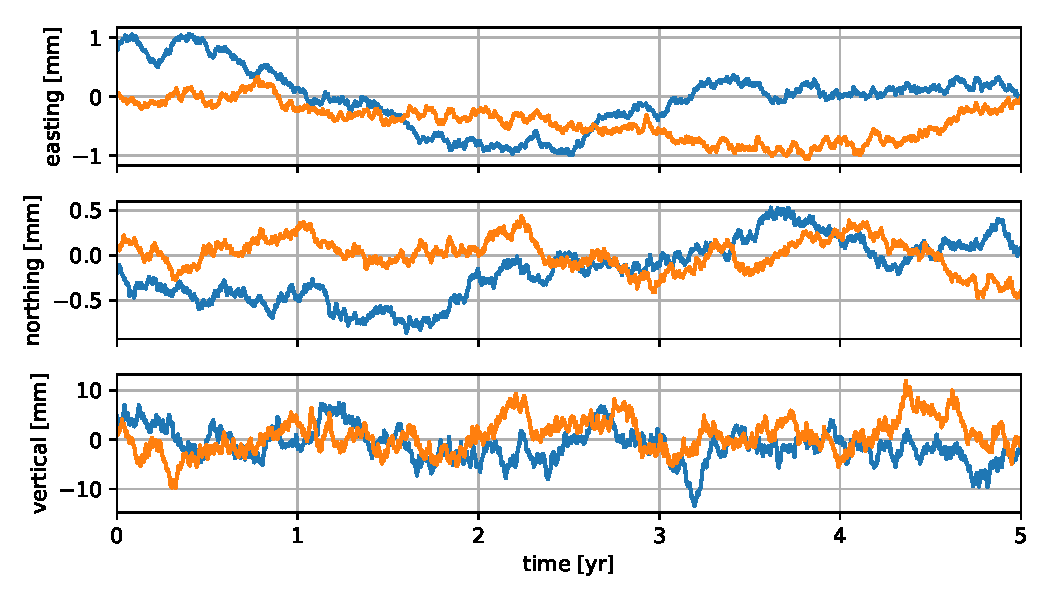
\includegraphics{figures/noise/noise-samples.pdf}
\caption{Two FOGM noise samples for each component. The FOGM hyperparameters have been set to the median values from Figure \ref{fig:NoiseParams}.}   
\label{fig:NoiseSamples}
\end{figure*}

Another significant source of noise in GNSS data is common mode error \citep[e.g.,][]{Wdowinski1997,Dong2006}, which is noise that is highly spatially correlated. When not accounted for, common mode error manifests as spatially uniform undulations in estimated transient displacements. However, estimated transient strain rates are insensitive to common mode error. We therefore do not include common mode error in our noise model. We then make the simplifying assumption that $\eta(p) = 0$ for the easting and northing component of GNSS data.  

\subsection{Prior model}\label{sec:SignalModel}
We next establish our prior model for transient displacements. Specifically, we discuss our choice for the covariance functions $X(\vec{x},\vec{x}')$ and $T(t,t')$. For $X$, we use the squared exponential (SE) covariance function,
\begin{equation}\label{eq:SE}
X(\vec{x},\vec{x}') = \exp\left(\frac{-||\vec{x} - \vec{x}'||_2^2}{2 \ell^2}\right).
\end{equation}
The SE covariance function is commonly used in kriging \citep[e.g,][]{Cressie1992} and Gaussian process regression \citep[e.g.,][]{Rasmussen2006}. The SE is a positive definite covariance function for any number of spatial dimensions. A Gaussian process with an SE covariance function is isotropic and has realizations that are infinitely differentiable. In terms of geodetic applications, \citet{Kato1998} and \cite{El-Fiky1999} demonstrated that the SE accurately describes the covariance of secular GNSS derived velocities in Japan.     

We consider three potential models for the temporal covariance of $u$. First, we consider the one-dimensional SE covariance function, 
\begin{equation}\label{eq:TimeSE}
T(t,t') = \phi^2\exp\left(\frac{-|t - t'|^2}{2\tau^2}\right).
\end{equation}
Note that $T$ includes the hyperparameter $\phi$, which serves to scale the covariance function $C_u$. Second, we consider integrated Brownian motion (IBM). IBM has zero mean and its covariance function can be found by integrating the covariance function for Brownian motion as
\begin{align}\label{eq:IBM}
T(t,t') &= \int_0^t \int_0^{t'} \phi^2 \min(s,s') \,ds'\,ds \\
        &= \frac{\phi^2}{2}\min(t,t')^2 \left(\max(t,t') - \frac{1}{3}\min(t,t')\right), \ \ \ t,t' \geq 0.
\end{align}
IBM has been used in the context of Kalman filtering as a non-parametric model for the time dependence of geophysical signals \citep[e.g.,][]{Segall1997,McGuire2003,Ohtani2010,Hines2016a}. It should be emphasized $t=0$ is a reference time at which the Gaussian process is exactly zero. For some geophysical signals, it is appropriate to have this reference time. For example, if we are trying to identify postseismic deformation then $t$ should be zero at the time of the earthquake.  However, if we are interesting in detecting transient events, where there is no known start time, then IBM may not be an appropriate prior, and an isotropic Gaussian process should be preferred. In the following analysis, we make the quite arbitrary choice that $t$ is zero on the first epoch of $\mitbf{d}_*$. Using an earlier reference time does not change the results discussed in this section. Our third option for $T$ is the Wendland class of covariance functions \citep{Wendland2005}. Wendland covariance functions have compact support and hence their corresponding covariance matrices are sparse. In our analysis, we exploit this sparsity with the CHOLMOD software package \citep{Chen2008}. Wendland functions are positive definite in $\mathbb{R}^d$, and they describes an isotropic Gaussian process with realizations that can be differentiated $k$ times. The form of the covariance function depends on the choice of $d$ and $k$. We use $d=1$ since we are describing the temporal covariance of $u$. We use $k=2$, giving samples of $u$ continuous velocities and accelerations. The corresponding Wendland covariance function is 
\begin{equation}\label{eq:Wendland}
T(t,t') = \phi^2\left(1 - \frac{|t - t'|}{\tau}\right)^5_+ \left(\frac{8|t - t'|^2}{\tau^2} + \frac{5|t - t'|}{\tau} + 1\right), 
\end{equation}
where
\begin{equation}
(t)_+ = 
\begin{cases}
t, \ \ \ t > 0 \\
0, \ \ \ \mathrm{otherwise}.
\end{cases}
\end{equation}

We next determine appropriate hyperparameters for $X$ and each of the three candidate covariance functions for $T$. First, we clean the GNSS datasets by removing offsets at times of equipment changes and removing outliers with the method describe in Section \ref{sec:Outlier}. For the outlier detection algorithm, our prior model, $u$, is chosen to have a length-scale and time-scale which is able to approximately describe SSE displacements. We use the SE covariance function for $X$ with length-scale $\ell = 100$ km, and we use the Wendland covariance function for $T$, due to its computational efficiency, with time-scale $\tau = 0.1$ yr and $\phi = 1$ mm.  The outlier detection algorithm is particularly effective at removing outliers for stations at high elevation (Figure \ref{fig:Outliers}), which can be adversely affected by ice or snow during the winter \citep{Lisowski2008}. After cleaning the dataset, we divide it into seven subsets which are four months long and each centered on the time of a SSE. The times of the seven SSEs are determined with tremor records from \cite{Wech2010}. We use the REML method to find the optimal hyperparameters for $T$ and $X$ for each subset of data. We choose to make each data subsets four months long because it is long enough to encompass a SSE in Cascadia, while it is short enough to still be computationally tractable. However, four months is too short to resolve the sinusoids in $\mitbf{d}$, and they are omitted from $\mitbf{d}$ in this REML analysis for Cascadia SSEs. The estimated hyperparameters for $u$ are summarized in Table 1. Based on the interquartile ranges, the estimated hyperparameters for the SE and Wendland covariance functions do not vary significantly between SSEs. This suggests that the median of estimated hyperparameters should be an appropriate prior model for all Cascadia SSEs. For the IBM model, there are several anomalously large values for $\ell$ and $\phi$, which results in large interquartile ranges.   

\begin{figure*}
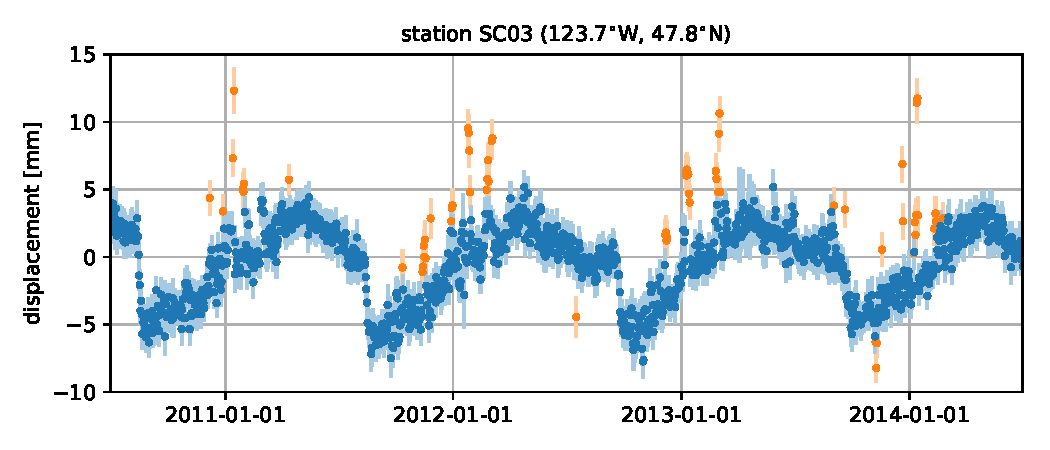
\includegraphics{figures/outliers/outliers.pdf}
\caption{Detrended easting component of displacements at station SC03, which is located on Mount Olympus in Washington. The orange markers indicate outliers that were automatically detected using the algorithm from Section \ref{sec:Outlier}. The error bars show one standard deviation uncertainties. Note that outliers tend be observed in the winter, suggesting that they were caused by snow or ice.}   
\label{fig:Outliers}
\end{figure*}

\begin{table}\label{tab:Parameters}
\caption{Optimal hyperparameters for the prior on transient displacements determined with the REML method. The temporal covariance function is indicated by the ``$T$'' column. The SE, IBM, and Wendland covariance functions are defined in eqs. (\ref{eq:TimeSE}), (\ref{eq:IBM}), and (\ref{eq:Wendland}), respectively. The spatial covariance function, $X$, is the squared exponential (eq. \ref{eq:SE}) in all cases. The hyperparameters are estimated for each of the seven SSEs considered in this study, and the tabulated values indicate the median and interquartile ranges of estimates. The ``diff $\log$(REML)'' column compares the log REML likelihood to the log REML likelihood when using the SE covariance function for $T$. Negative values indicate that observations are more consistent with the SE covariance function.} 
\begin{tabular} {l l l l l l}
$T$ & direction & $\ell$  & $\phi$   & $\tau$  & diff. $\log$(REML) \\ \hline
SE & east   & 92 $\pm$ 25 km  & 0.62 $\pm$ 0.11 mm  & 0.026 $\pm$ 0.011 yr  &  - \\
SE & north  & 91 $\pm$ 53 km  & 0.43 $\pm$ 0.05 mm  & 0.030 $\pm$ 0.017 yr  &  - \\
Wendland & east   & 95 $\pm$ 30 km  & 0.66 $\pm$ 0.15 mm  & 0.093 $\pm$ 0.044 yr &  0.78 $\pm$ 0.87 \\
Wendland & north  & 92 $\pm$ 57 km  & 0.46 $\pm$ 0.10 mm  & 0.116 $\pm$ 0.057 yr &  0.08 $\pm$ 0.58 \\
IBM & east   & 110 $\pm$ 130 km & 290 $\pm$ 420 mm/yr$^{1.5}$  & -          & -16.4 $\pm$ 7.8 \\
IBM & north  & 150 $\pm$ 560 km & 110 $\pm$ 250 mm/yr$^{1.5}$ & -           & -10.1 $\pm$ 2.3 \\
\end{tabular}
\end{table}

Next we identify which covariance function for $T$ best describes the SSEs. One approach is to compare the REML likelihoods for each covariance function, similar to the analysis in \citet{Langbein2004}. In Table 1, we summarize how the log REML likelihoods for the Wendland and IBM covariance functions compare to the SE covariance function.  Based on the differences in log REML likelihoods, the data is substantially more likely to come from a Gaussian process with a SE or Wendland covariance function than an IBM covariance function. The REML likelihoods do not definitively indicate whether the SE or Wendland covariance function is preferable. 

To further explore which covariance function for $T$ best describes SSEs, we compare the observations to the predicted displacements for each covariance function. We consider the data prediction vector to be $\hat{\mitbf{d}} = \left(u(\mitbf{P}) + \mitbf{G}\mitbf{a}\right)|\mitbf{d}_*$. Following a similar procedure as in Section \ref{sec:Method}, it can be shown that $\hat{\mitbf{d}}$ is normally distributed with mean 
\begin{equation}\label{eq:DataPredMean}
\mitbf{\mu}_{\hat{d}} = \left[\begin{array}{cc}
                           C_u(\mitbf{P},\mitbf{P}) & \mitbf{G} \\
                           \end{array}\right]
                     \left[\begin{array}{cc}
                           \mitbf{\Sigma} & \mitbf{G} \\
                           \mitbf{G}^T  & \mitbf{0} \\
                           \end{array}\right]^{-1}
                     \left[\begin{array}{c}
                           \mitbf{d}_* \\
                           \mitbf{0} \\
                           \end{array}\right]
\end{equation}  
and covariance
\begin{equation}\label{eq:DataPredCov}
\mitbf{C}_{\hat{\mitbf{d}}} = C_u(\mitbf{P},\mitbf{P}) - 
                        \left[\begin{array}{cc}
                              C_u(\mitbf{P},\mitbf{P}) & \mitbf{G} \\
                              \end{array}\right]
                        \left[\begin{array}{cc}
                              \mitbf{\Sigma} & \mitbf{G} \\
                              \mitbf{G}^T  & \mitbf{0} \\
                              \end{array}\right]^{-1}
                        \left[\begin{array}{c}
                              C_u(\mitbf{P},\mitbf{P}) \\
                              \mitbf{G}^T \\
                              \end{array}\right].
\end{equation}
We compute $\hat{\mitbf{d}}$ using SE, Wendland, and IBM covariance functions for $T$ and the median hyperparameters from Table 1. Figure \ref{fig:Fit} compares the easting component of $\mitbf{d}_*$ to $\hat{\mitbf{d}}$ for the winter 2015-2016 SSE at station P436, which is among the stations that record the strongest signal. The data prediction vector reasonable fits the displacements throughout the SSE, regardless of the choice of $T$. The prediction for the IBM covariance function contains slightly more high frequency, and perhaps spurious, features. The predictions for the Wendland and SE covariance functions are nearly indistinguishable. Overall, the predicted displacements are not strongly sensitive to the choice of temporal covariance function. In our estimates of transient strain discussed in the next section, we ultimately settle on the Wendland covariance function for $T$ and use the median values from Table 1 for the hyperparameters. We choose the Wendland covariance function over the SE covariance function because of its computational advantages.     

\begin{figure*}
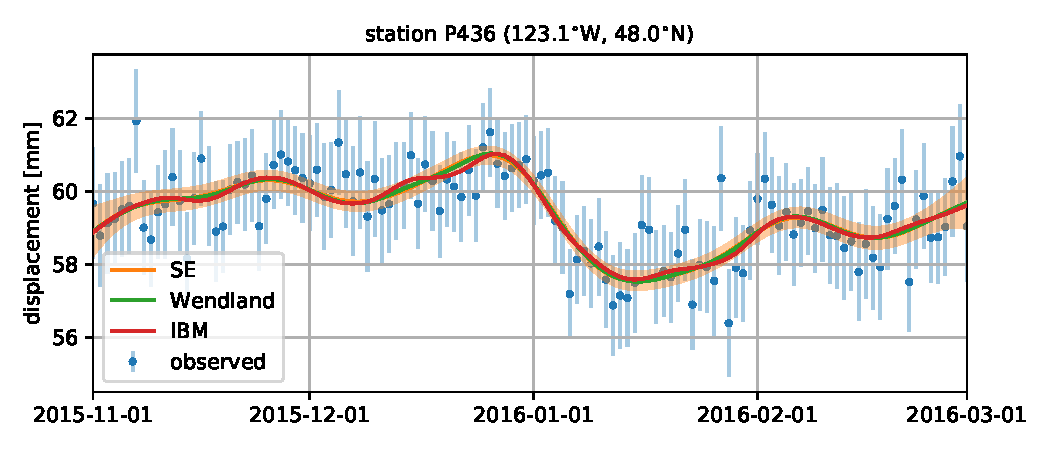
\includegraphics{figures/signal_fit/signal-fit.pdf}
\caption{Observed easting component of displacements at station P436 and predicted displacements when using different covariance functions for $T$. The one standard deviation uncertainties are shown for the observations and the predicted displacements when using the SE covariance function. For clarity, uncertainties are not shown for the IBM and Wendland covariance functions, but they are nearly equivalent to the uncertainties for the SE covariance function.}   
\label{fig:Fit}
\end{figure*}

\subsection{Transient Strain Rates}\label{sec:Results} 
Having established a noise model and a prior for transient displacements, we use the cleaned GNSS dataset to calculate transient strain rates in the Puget Sound region.  We calculate transient strain rates for each day from January 1, 2010 to May 15, 2017. The strain rates are estimates at a grid of points spanning the study area. In Figure \ref{fig:StrainMap} we show the transient strain rates on January 1, 2016, which coincides with the height of an SSE. We have included an animation showing the map view of strain rates through time as supplementary material. The strain rates shown in Figure \ref{fig:StrainMap} are generally similar to the strain rates for the other six SSEs considered in this study. The SSEs cause compression in the Olympic Peninsula and extension east of Puget Sound. For comparison, estimated secular strain rates indicate trench perpendicular compression throughout this study region \citep{Murray2000,McCaffrey2007,McCaffrey2013}. The SSEs are thus concentrating tectonically accumulated strain energy trench-ward, and presumably pushing the subduction zone closer to failure. Similar conclusions have been drawn based on fault slip models \citep[e.g.,][]{Dragert2001,Wech2009,Schmidt2010}, which reveal that SSEs are occurring down-dip of the seismogenic zone and migrating stress upward. A key difference between the strain inferred here and strain that can be derived from fault slip models is that our estimated strain rates are not based on an assumed physical model. In contrast, fault slip models can be biased by errors in the assumed fault geometry or lithospheric rheology. Moreover, the degrees of freedom in fault slip models usually cannot be constrained by GNSS data alone, and it is necessary to impose regularization which further biases the results. Since our estimated strain rates lack such systematic errors, we can be more confident that our solution is unbiased and has meaningful uncertainties.  

\begin{figure*}
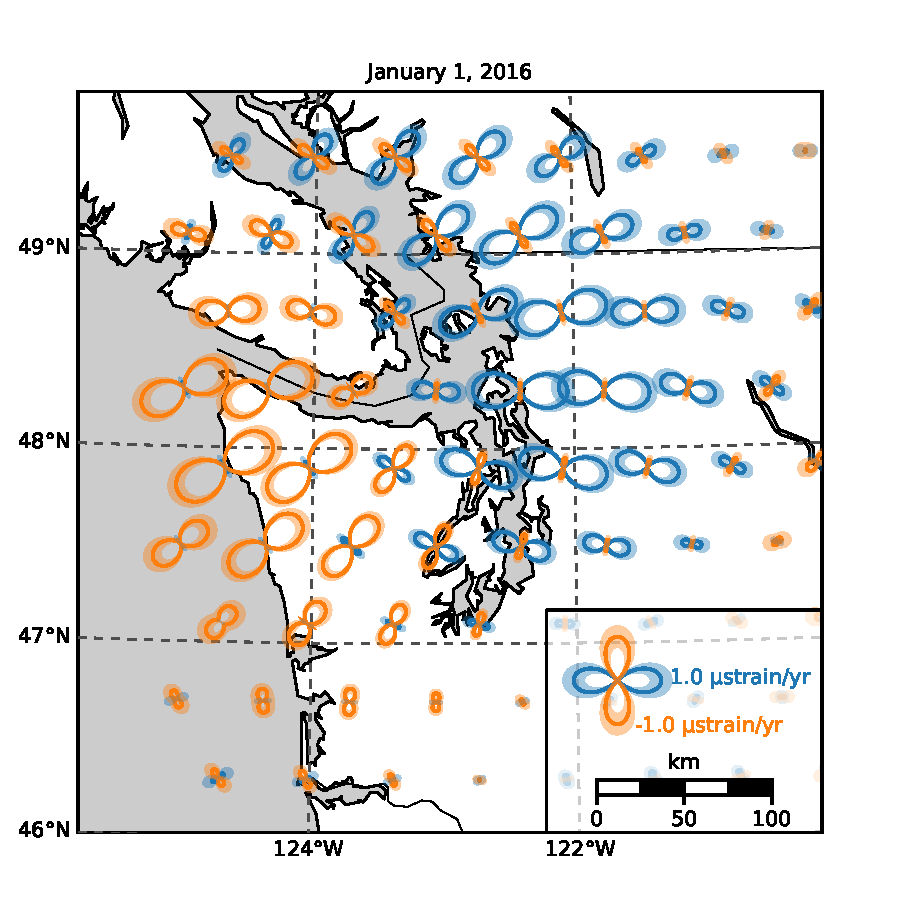
\includegraphics{figures/strain_map/strain-map.pdf}
\caption{Estimated transient strain rates during the Winter 2015-2016 SSE. Strain glyphs show the normal strain rate along each azimuth, where orange indicates compression and blue indicates extension. The shaded regions indicate one standard deviation uncertainties in the normal strain rates.}   
\label{fig:StrainMap}
\end{figure*}

In Figure \ref{fig:StrainTs} we show the time dependence of estimated transient strain rates at a position on the Olympic Peninsula, where transient strain rates from SSEs are largest. To verify that the estimated transient strain rates are accurately identifying geophysical signal, we compare the signal-to-noise ratio from eq. (\ref{eq:SNR}) to the frequency of seismic tremor (Figure \ref{fig:StrainMag}). A signal-to-noise ratio greater than ${\sim}3$ can be interpreted as a detected geophysical signal. For each detected event there is a corresponding peak in seismic tremor. We are also able to clearly identify transient strain associated with a more subtle SSE in August 2014. In between peaks in seismic tremor, the signal-to-noise ratio is consistently between 0 and 2, suggesting that all the transient strain detected at this location is associated with SSEs.

\begin{figure*}
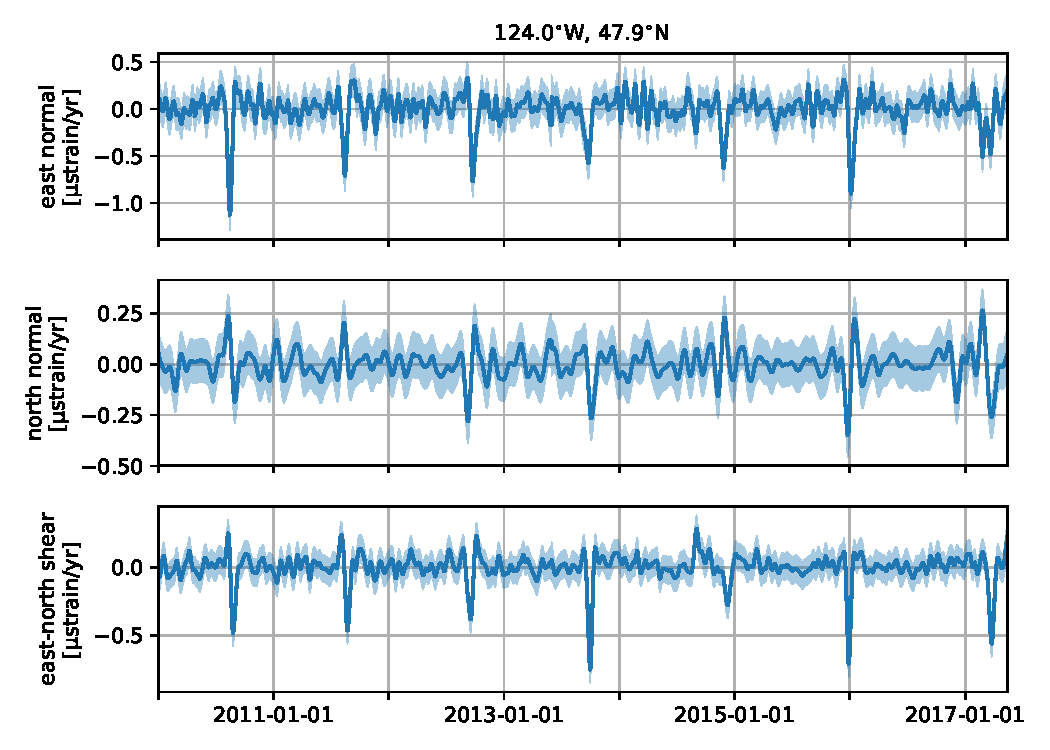
\includegraphics{figures/strain_ts/strain-ts.pdf}
\caption{Three components of the transient horizontal strain rate tensor estimated at the position shown in Figure \ref{fig:Context}. The shaded regions indicate one standard deviation uncertainty.}   
\label{fig:StrainTs}
\end{figure*}

\begin{figure*}
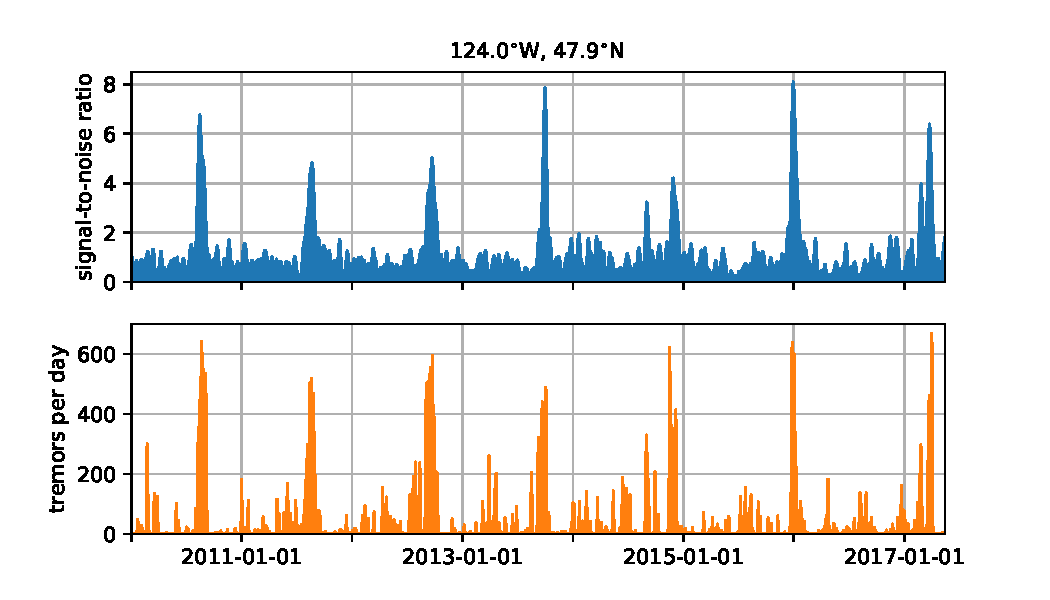
\includegraphics{figures/strain_ts/mag-ts.pdf}
\caption{(top) Signal-to-noise ratio (eq. \ref{eq:SNR}) at the position shown in Figure \ref{fig:Context}. (bottom) Frequency of tremors in the region shown in Figure \ref{fig:Context}.}   
\label{fig:StrainMag}
\end{figure*}

The results we have presented thus far indicate that we are identifying the strain that we should expect to see. There are, however, features in our estimated transient strain rates which we were not expecting. For example, there is a brief period of east-west extension on the Olympic peninsula several days prior to some of the SSEs. This feature can be seen before the summer 2012 and winter 2015-2016 SSEs in Figure \ref{fig:StrainTs} as well as in the supplementary animation. A discussion on the mechanisms causing this deformation is outside the scope of this study.

\section{Discussion}\label{sec:Discussion}
We have demonstrated that transient strain rates estimated with the method described in Section \ref{sec:Method} can be used to detect SSEs and will be robust to detect other transient geophysical phenomena. Another potential application would be to use GNSS derived transient strain rates to better understand the data from borehole strain meters (BSMs). The Plate Boundary Observatory maintains 43 BSMs in Cascadia, and it has been demonstrated that BSMs are able to record transient geophysical events such as SSEs \citep[e.g.,][]{Dragert2011}. However, there are complications that prevent BSM data from being used quantitatively in geophysical studies. One difficulty is that BSM data should be calibrated with a well known strain source, such as diurnal and semidiurnal tides \citep{Hart1996,Roeloffs2010,Hodgkinson2013}. Unfortunately, the tidal forces at BSMs which record SSEs are strongly influenced by local bodies of water such as the Straight of Juan de Fuca, making it difficult to form a theoretical prediction of tidal strains \citep{Roeloffs2010}. Another complication is that noise in BSM data is not well understood. The noise consists, in part, of a long-term decay resulting from the instrument equilibrating with the surrounding rock \citep{Gladwin1987}. Typically, this noise is dealt with in an ad-hoc manner by fitting and removing exponentials and low-order polynomials. We envision that the GNSS derived strain rates from this paper can be used as a reference strain for calibrating BSM data and quantify its noise.    

There is potential for a more thorough analysis of the spatio-temporal noise in GNSS data, $\eta$, than what was performed in Section \ref{sec:NoiseModel}. We did not explore the spatial covariance of $\eta$. Spatially correlated common mode noise, which results from factors such as reference frame error, is a non-negligible component of GNSS data. We ignore common mode error in this study because transients strain rates are insensitive to it. For other geophysical studies based on GNSS data, such as fault slip inversions, it may be necessary to incorporate a spatially covarying noise model \citep[e.g.,][]{Miyazaki2003}. We can also improve upon the seasonal model used in this study, which consists of four spatially uncorrelated sinusoids for each station. We did not explore the spatial covariance of seasonal deformation or the temporal roughness (i.e., the number of sinusoids needed to describe the observations). The periodic Gaussian process \citep{Mackay1998} is an alternative model for seasonal deformation and is well suited for exploring the roughness of seasonal deformation.  The periodic Gaussian process has zero mean and the covariance function
\begin{equation}\label{eq:Periodic}
T(t,t') = \phi^2 \exp\left(\frac{-\sin(\pi|t - t'|)^2}{2\tau^2}\right).
\end{equation}
Realizations have annual periodicity and the roughness is controlled by $\tau$. Decreasing $\tau$ has the same effect as including higher frequency sinusoids in the seasonal model. The optimal value for $\tau$ can be found with the REML method as described in Section \ref{sec:NoiseModel}. 

The transient strain rates estimated in this study are constrained by about seven years of daily displacement observations from 94 GNSS stations. It can be computationally intensive to evaluate eqs. (\ref{eq:PosteriorMean3}) and (\ref{eq:PosteriorCov3}) for a dataset with this size. We significantly reduce the amount of memory needed to estimate transient strain rates by describing the temporal covariance of displacements with a compact Wendland covariance function. Using a compact covariance function for our prior turns eqs. (\ref{eq:PosteriorMean3}) and (\ref{eq:PosteriorCov3}) into sparse systems of equations, which we then solve with CHOLMOD. CHOLMOD is designed for solving sparse, positive definite systems of equations. The matrix being inverted in eqs. (\ref{eq:PosteriorMean3}) and (\ref{eq:PosteriorCov3}) is not positive definite; however, we can use another partitioned matrix inversion identity from \citet{Press2007} to partition it into positive definite submatrices to be inverted. Even when using a compact covariance function, it may still be necessary to reduce the computational burden by dividing the data into subsets and evaluating transient strain rates for each subset.   

\section{Conclusion}\label{sec:Conclusion}
In this paper we propose using Gaussian process regression (GPR) to estimate transient strain rates from GNSS data. Most other methods for estimating strain rates assume a parametric representation of deformation, which can bias the results if the parameterization is not chosen carefully. Here we assume a stochastic, rather than parametric, prior model for displacements. Our prior model describes how much we expect transient displacements to covary spatially and temporally. If we know nothing about the underlying signal that we are trying to recover, then the prior model can be chosen objectively with maximum likelihood methods. Because GPR is a Bayesian method, the uncertainties on our estimated transient strain rates are well quantified, allowing one to discern geophysical signal from noise. We demonstrate that GPR is an effective tool for detecting geophysical phenomena, such as slow slip events, in our application to GNSS data from Cascadia. One limitation with GPR is that it is not robust against outliers. To overcome this limitation, we have introduced an effective pre-processing method for identifying and removing outliers from GNSS datasets. Another complication with GPR is that it usually involves inverting a dense matrix where the number of rows and columns is equal to the number of observations. This is prohibitive when using several years of daily GNSS observations from a network of several hundred stations. We significantly reduce the computational burden of GPR by using compact Wendland covariance function to describe our prior model. While this paper just focuses on estimating transient strain rates, we believe that GPR is a powerful tool that can be applied to a wide range of geophysical problems.   

\section{Acknowledgements}
This material is based upon work supported by the National Science Foundation under grant EAR 1245263. The EarthScope Plate Boundary Observatory data is provided by UNAVCO through the GAGE Facility with support from the National Science Foundation (NSF) and National Aeronautics and Space Administration (NASA) under NSF Cooperative Agreement EAR-1261833. An implementation of the method described in this paper is named Python-based Geodetic Network Strain software (PyGeoNS). PyGeoNS is distributed under the MIT License and can be found at www.github.com/treverhines/PyGeoNS. 

\bibliographystyle{gji}
\bibliography{mybib}  

\end{document}
